\section{Анализ алгоритма}

\subsection{Принцип работы}

Алгоритм является поиском максимума в массиве.
Программа:
\begin{enumerate}
    \item Выделяет память под массив, инициализирует генератор случайных значений;
    \item Заполняет массив случайными числами;
    \item Ищет максимум с определенными настройками \textit{OpenMP}.
\end{enumerate}

Поиск максимума осуществляется параллельно. 
Массив разбивается на секции (почти) равного размера, которые распределяются между потоками.
Распределение зависит от параметра \textit{schedule}, который здесь не указан.
В таком случае он определяется компилятором/ОС.

Временная сложность алгоритма $O(\frac{n}{p})$, где:
\begin{itemize}
 \item $n$ -- число элементов в массиве;
 \item $p$ -- число используемых потоков.
\end{itemize}

Блок-схема однопоточного исполнения алгоритма выглядит следующим образом:\\
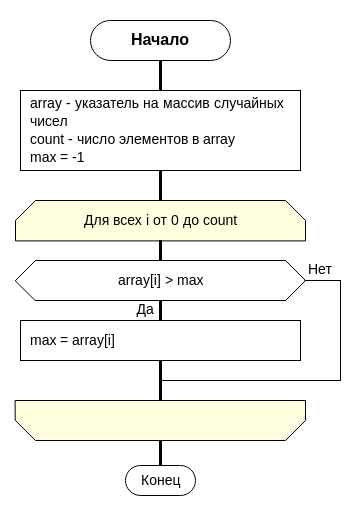
\includegraphics[scale=0.6]{res/flowchart.png}

\subsection{Директивы \textit{OpenMP}}

Поясним представленные директивы \textit{OpenMP}.

Директива \textit{parallel} задает опции параллелизации:
\begin{itemize}
    \item \textit{num\_threads} -- число потоков;
    \item \textit{shared} -- общая для потоков память;
    \item \textit{reduction} -- способ объединения локальных переменных в глобальную. В данном случае вычисление максимума;
    \item \textit{default} -- локальность переменных \textit{по умолчанию}. В данном случае все переменные по умолчанию локальные.
\end{itemize}
Если бы данной директивы не было, то следующий за ней блок кода исполнялся бы одним потоком без участия \textit{OpenMP}. 

Директива \textit{for} используя опции, задаваемые директивой \textit{parallel} распределяет итерации цикла между потоками.
Если бы данной директивы не было, то цикл, следующий за ней, выполнился бы во всех потоках (не было бы распределения итераций).
